% Template for the Journal of Computational Science and Applications (JCSA)
% Published by the University of Lahore -- ISSN 2710-3102
% Official author guidelines: https://journals.uol.edu.pk/JCSA/Author-Guideline
\documentclass[twoside,10pt]{article}
\raggedbottom
\usepackage{lipsum}  % For sample/placeholder text
\usepackage{fancyhdr}
\usepackage{geometry}
\usepackage{multicol}
\usepackage{abstract}
\usepackage{graphicx}
\usepackage{caption}
\usepackage{titlesec}
\usepackage{ragged2e}  % Provides the justifying command
\usepackage{amssymb}  % For additional symbols
\usepackage{parskip}  % Automatically handles paragraph spacing
\usepackage{amsmath}  % For advanced math environments
\usepackage{newtxtext}  % Times New Roman font
\usepackage{booktabs}  % For improved table appearance
\usepackage{array}     % For customizing table columns
\usepackage{graphicx}
\usepackage{subcaption}
\usepackage{float}


% The starting page number is normally assigned by the editorial office
% once the article is scheduled into a specific issue. Authors can leave
% this at 1; production will update it if required.
\setcounter{page}{1}

% Define custom column types for better alignment and spacing
% \newcolumntype{L}[1]{>{\raggedright\arraybackslash}p{#1}} % Left aligned column
% \newcolumntype{C}[1]{>{\centering\arraybackslash}p{#1}}   % Center aligned column
% \newcolumntype{R}[1]{>{\raggedleft\arraybackslash}p{#1}}  % Right aligned column

\usepackage[font=footnotesize, labelfont=bf, justification=raggedright, format=plain]{caption}

\captionsetup[table]{
    labelsep=period,               % Period after label for tables
    justification=raggedright      % Ensure left alignment of captions
}

\captionsetup[figure]{
    labelsep=period,               % Period after label for figures
    justification=raggedright      % Ensure left alignment of captions
}

\usepackage[backend=bibtex,style=ieee]{biblatex}
\addbibresource{references.bib}  % Add your .bib file
% Customizing bibliography heading
\defbibheading{bibliography}[\refname]{%
  \section{\MakeUppercase{REFERENCES}}}

% Set page margins
\geometry{
    a4paper,
    left=0.8in,
    right=0.8in,
    top=1in,
    bottom=1in
}

% % Increase space between columns
% \setlength{\columnsep}{15pt}

% Define the centred abstract heading
\renewcommand{\abstractname}{\hspace{1.3em}\textbf{Abstract}}

\titleformat{\section}{\large\bfseries\uppercase}{\thesection.}{1em}{}

\titleformat{\subsection}{\normalfont\bfseries\flushleft}{\thesubsection.}{1em}{}

\titleformat{\subsubsection}{\normalfont\bfseries\itshape\flushleft}{\thesubsubsection}{1em}{}

% Set font sizes for abstract
\renewcommand{\abstractnamefont}{\normalfont\fontsize{14}{20}\bfseries}
\renewcommand{\absnamepos}{flushleft}
\renewcommand{\abstracttextfont}{\normalfont\fontsize{11}{13}\selectfont}

% Keywords environment
\newcommand{\keywordsname}{Keywords}
\newenvironment{keywords}
  {\par\noindent\hspace{2em}\textbf{\keywordsname:}}
  {\par}

\hyphenpenalty=10000
\exhyphenpenalty=10000
\sloppy

% Set up header and footer styles
\pagestyle{fancy}
\fancyhf{}  % Clear default header and footer

% Odd page headers -- replace with a short running form of your title
\fancyhead[R]{\small Institute for Computing in Research}

% Footer: Page numbers only (on all pages except the first one)
\fancyfoot[C]{\thepage}

\title{\fontsize{16}{20}\selectfont\textbf{Identifying Lunar Skylight Candidates with Object Detection}}
\author{
    \fontsize{12}{14}\selectfont
    Nao Joy
}
\date{\today}

\begin{document}
% Change "Research Article" to the appropriate article type if needed
% (e.g. Review Article, Short Communication).
\vspace{-0.5cm}  % Adjust spacing as needed between header and "Research Article"

% Now, insert the title and the author information
\maketitle

\begin{abstract}
\fontsize{12}{14}\selectfont
\vspace{1em}
\justifying
% \textit{[Replace this paragraph with your abstract. The abstract should be a single, self-contained paragraph of approximately 150--250 words summarizing the purpose of the study, the methodology used, the principal results, and the main conclusions. Avoid citations, footnotes, and undefined abbreviations in the abstract.]}
This is a project for creating an object detection model and identifying lunar skylight candidates, which are potential locations for future lunar bases. Since lunar skylights are a subcategory of lunar pits and it's difficult to distinguish the two from each other, the model detects candidates that can be reviewed by humans. I downloaded images taken by the Lunar Reconnaissance Orbiter's narrow angle camera and processed them to create my training dataset. I then trained a YOLO \cite{Jocher_Ultralytics_YOLO26_Unified_2026} object detection model on this dataset. I then ran inferences on images by dividing them into smaller 640x640 pixel tiles and running the trained model on them.

\end{abstract}

\vspace{1cm}

\section{Introduction}
\fontsize{13}{15}\selectfont
% \textit{[Replace this section with your Introduction. Provide sufficient background to place the work in context, state the problem being addressed, and summarize the objectives and contributions of the study. The example paragraph below shows the default paragraph style, justification, and hyphenation settings used throughout the template.]}

%TODO: explain object detection

The recent Artemis missions have setup an exciting pipeline for sending people back to the moon and eventually creating research bases. However, this comes with potential dangers to consider. Unlike Earth, the moon has no atmosphere, so the surface is a lot more vulnerable to solar radiation, and the temperature is variable. For humans who are used to living on Earth and its milder climate, the moon is a hostile environment. Lava tubes offer a potential solution to this problem, as below the surface, the temperature can be controlled more easily and the tunnels are protected from solar radiation. Lunar pits occur when lava collapses sections of the moon's surface. Lunar skylights are a type of lunar pits that are entrances to these lava tubes, which is why it is important to search for them. In order to survive the harsh conditions, we have to become like ants on the moon and live in those tunnels.

In this project, I used object detection to identify lunar skylight candidates (lunar pits and skylights are difficult to distinguish). Due to the limited number of previously identified lunar pits, my model didn't have much data to train on. Thus, rather than identifying lunar pits with near-perfect accuracy, the goal was to identify candidates that looked like pits and could be later checked by humans. Even if the model ended up detecting objects that were actually craters or boulders, it wouldn't be as bad as glossing over many lunar pits.

% In-text citations use the \verb|\cite| command and follow the IEEE numbered style configured for this template, e.g., a single reference \cite{1_Su2022} or multiple references \cite{2_Lind2021, 3_Kuwahara2022}.

\section{Methodology}
% \textit{[Replace this section with a description of your data sources and methodology.]}
\fontsize{13}{15}\selectfont
I downloaded all of my images from the Lunar Orbital Data Explorer \cite{lroc_nac_data}. I found a list of identified lunar pits from the Lunar Pit Locations shapefile \cite{lroc_pit_csv}. This website provided a csv containing image ids corresponding to the pits and metadata, such as geospatial information and pit coordinates. I wrote Python code to extract important information from the csv, such as the pit image IDs and the pit coordinates. To generate labels for my images, I used the Segment Anything Model (SAM) \cite{kirillov2023segany}.

\subsection{Dataset Creation}
\fontsize{12}{14}\selectfont
% \textit{[Use subsections to organize the methodology, e.g., data description, variable construction, and model specification.]}

\subsubsection{Downloading Images}
Due to the large size of the raw files (approx. 500 MB per file), I had to store the data on an external drive rather than my computer. I chose to download pre-calibrated images, because during previous testing, I had to process raw images with ISIS tools and SPICE data, which took a long time (several minutes per image) and took up even more storage (1 GB per image). The narrow range of angles from which the images were taken provided uniformity so the model had less information it had to train on.

\subsubsection{Converting and Cropping Images}
The files were initially stored as raw IMG files, so I had to take steps to convert them to formats compatible with the YOLO model. I first converted the IMG files to tiff files to preserve the image quality. The tiff images were very large (5064x52224 pixels), so I had to crop them to 640x640 pixel tiles and I further converted them to png files so the YOLO model could train on them. For processing the images and cropping them, I used the Numpy \cite{2020NumPy-Array} library to slice sections of images. On top of cropping the images around their pits, I randomly cropped the images by adding a random offset so the pits would be randomly placed in the resulting image, rather than being consistently centered. I confirmed that these cropped images didn't contain any pits by writing a function based on the PitScan \cite{wagner2018pitscan} algorithm, which examines the number of shadowed pixels in a potential pit and how they're oriented. The function I wrote created a base threshold for what pixels would be treated as shadows, then looked for a certain density of shadowed pixels in the image. This introduced variation into the dataset so the model wouldn't be trained to expect pits in the center of images. I also calculated the new pit coordinates relative to the cropped images with the random offsets and stored them in csv files. Additionally, I cropped random sections from the original tiff images to get background images without any pits. But I wanted to be confident that the cropped images didn't include any pits, as they would've skewed the model towards predicting images were backgrounds instead of containing pits. This greatly reduced the chance of false positives by training a model that wouldn't expect a pit in every image.

\subsubsection{Labeling Images}
After getting the randomly cropped pngs, I read the corresponding pit coordinate csv files and fed them to SAM to generate masks around the pits. SAM generates image overlays, which I then draw on the images with the OpenCV library \cite{opencv_library}, but the YOLO model expects text files with floats, so I normalized the masks and wrote them to text files. When I previously directly fed the images to SAM, it generated masks around many objects, such as boulders and craters, threw off the data I passed into the dataset. But feeding the pit coordinates improved SAM's accuracy and saved time. However, even with the pit coordinates, the SAM model didn't always create satisfactory labels, so I used Matplotlib \cite{Hunter_Matplotlib_A_2D_2007} to display three different labels per image and prompt the user for the best one. After labeling the images, I wrote a script to choose 15\% as many background images as pit images. Although including background images is important, the pits only take up dozens of pixels, so too many background images would skew the model. With a more balanced ratio of pit and background images, I then split them into training, testing and validation sets.

\subsection{Model Training and Implementation}
\fontsize{13}{15}\selectfont
%TODO: explain YOLO, back-propagation, classification, segmentation, etc.
I trained the YOLO object detection model on the split data. The model learned patterns from the training images and created initial weights. It then tested the weights on the testing images and after judging itself on the accuracy, it used back-propagation to update the weights. After training and finalizing the weights, the model then tested itself on the validation images to get final accuracy metrics. This process returned a folder of graphs; which showed accuracy metrics on classification, segmentation, drawing bounding boxes, etc.; and the final weights of the model. With the final weights, I tested the model on new images to search for new pits. Since I wasn't able to use the column 2 and 3 images in the initial training, running inferences on them with the model was basically a second instance of validation. Since the raw images are 5064x52224 pixels, I couldn't exactly pass each entire image into the model. Instead, I divided each image into smaller 640x640 pixel images that would take less memory and time to process. This ended up taking approximately 20 seconds per image, which was quite short considering the image size. This was made possible by the quick speed of the YOLO model.

\section{Results}

% \textit{[Replace this section with your results and discussion. The example figures and table below demonstrate the recommended formatting for graphical and tabular content in this template.]}
In the end, the model didn't have a great accuracy score. It could only accurately identify approximately 60\% of lunar pits, and it struggled with false positives, or falsely predicting an image contained a pit when it was just a background image.

\begin{figure}[H]
\centering
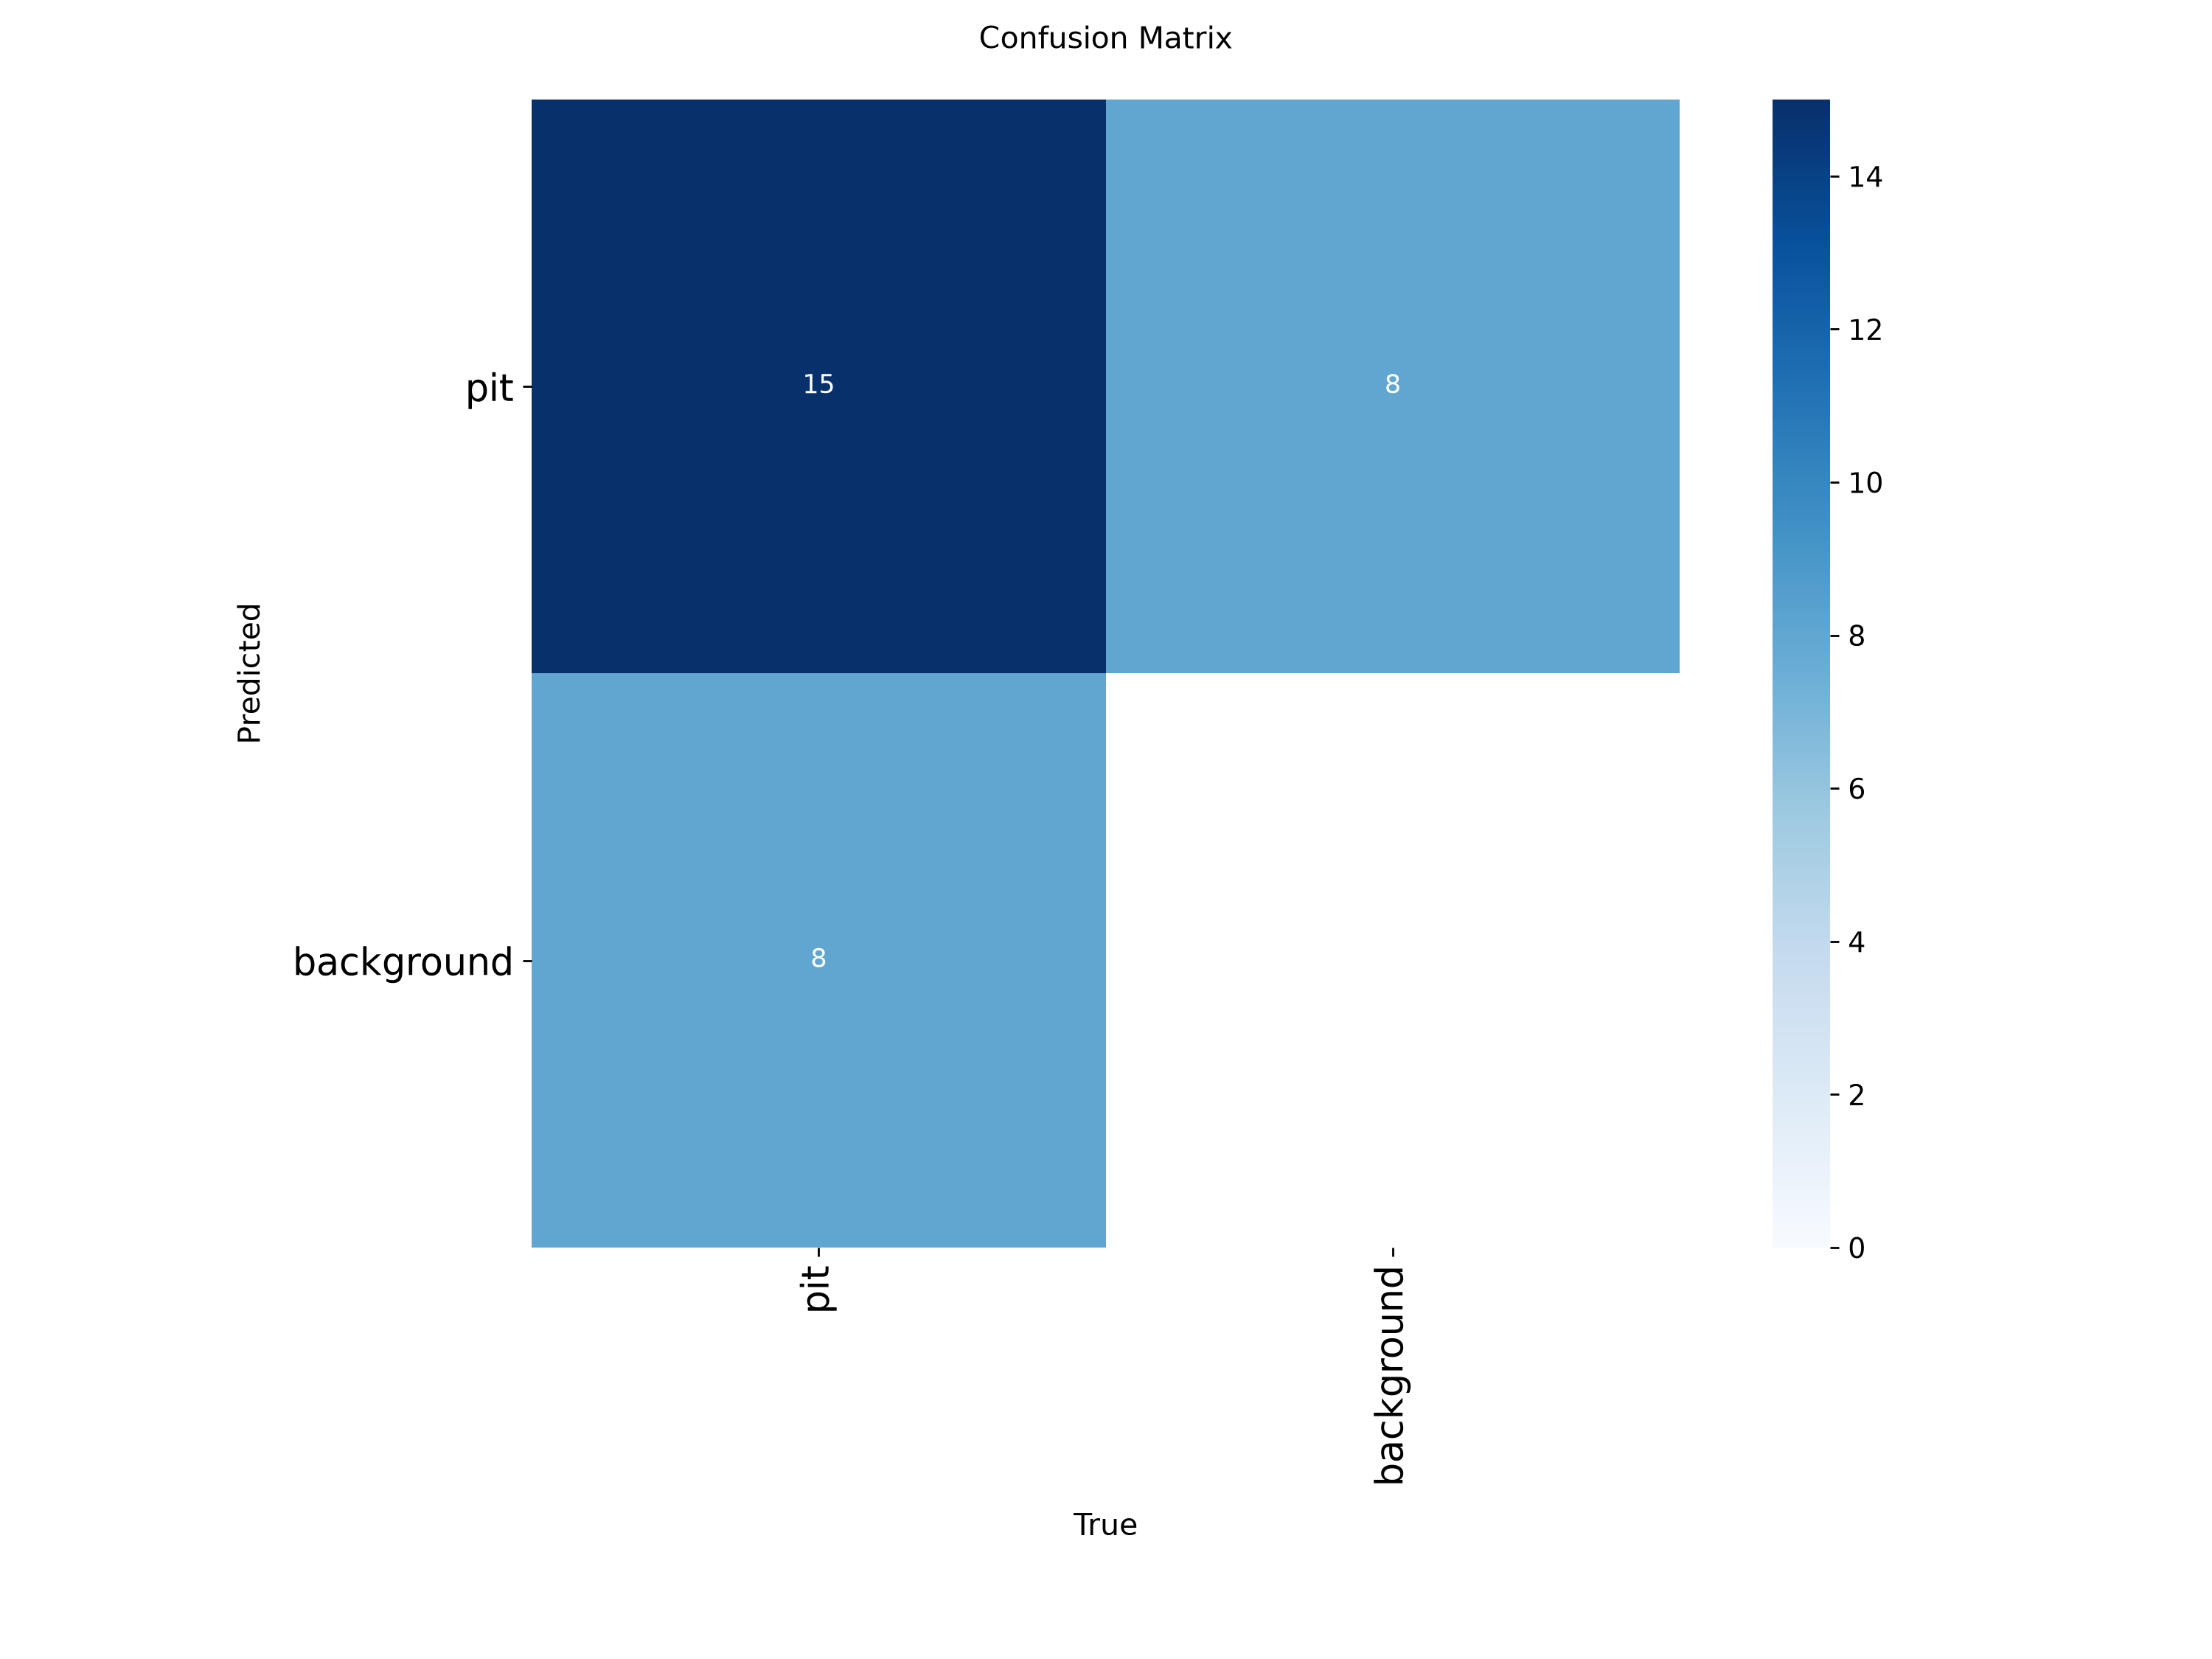
\includegraphics[width=0.5\textwidth]{images/confusion_matrix.png}
\caption{Confusion matrix showing predictions on pit and background images}
\label{fig:example-one}
\end{figure}

In the above confusion matrix, the model's predictions based on the testing images are shown on the left and the actual classes are shown on the bottom. Out of the 23 pit images, 15, or 65\%, were correctly predicted to contain pits. Out of the 8 background images, none of them were correctly predicted to be background images.

\begin{figure}[H]
    \centering
    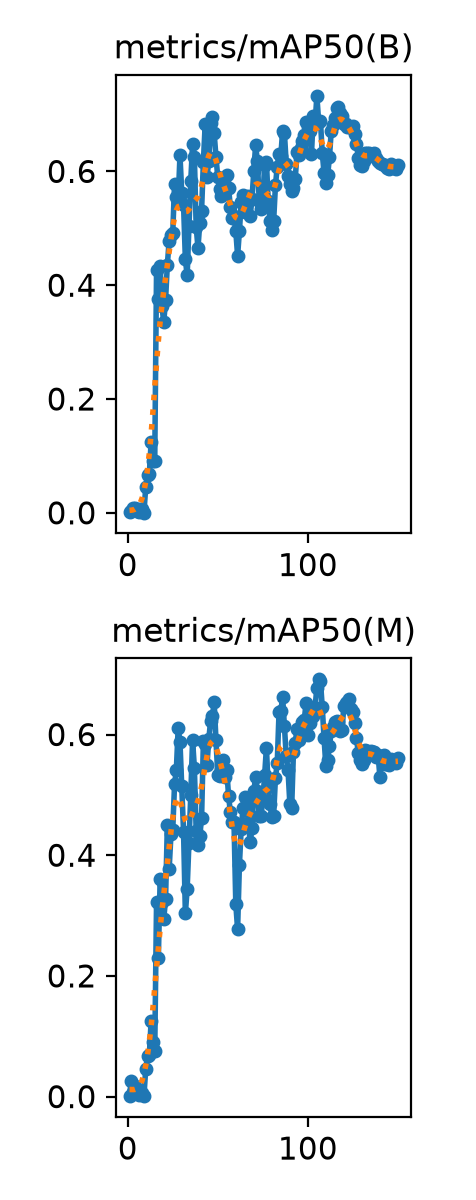
\includegraphics[width=0.5\linewidth]{images/metrics.png}
    \caption{Caption}
    \label{Metrics}
\end{figure}

Average precision (AP) measures the model's average precision. The model improved slightly more consistently for boxes (B) than masks (M), but both were oscillating around a general curve approaching a horizontal asymptote. However, this result can be explained by the lack of data, as getting an image or two wrong can significantly drop the precision, whereas a more robust dataset would be more resilient.

\begin{figure}[htbp]
  \centering
  \begin{subfigure}[b]{0.45\textwidth}
    \centering
    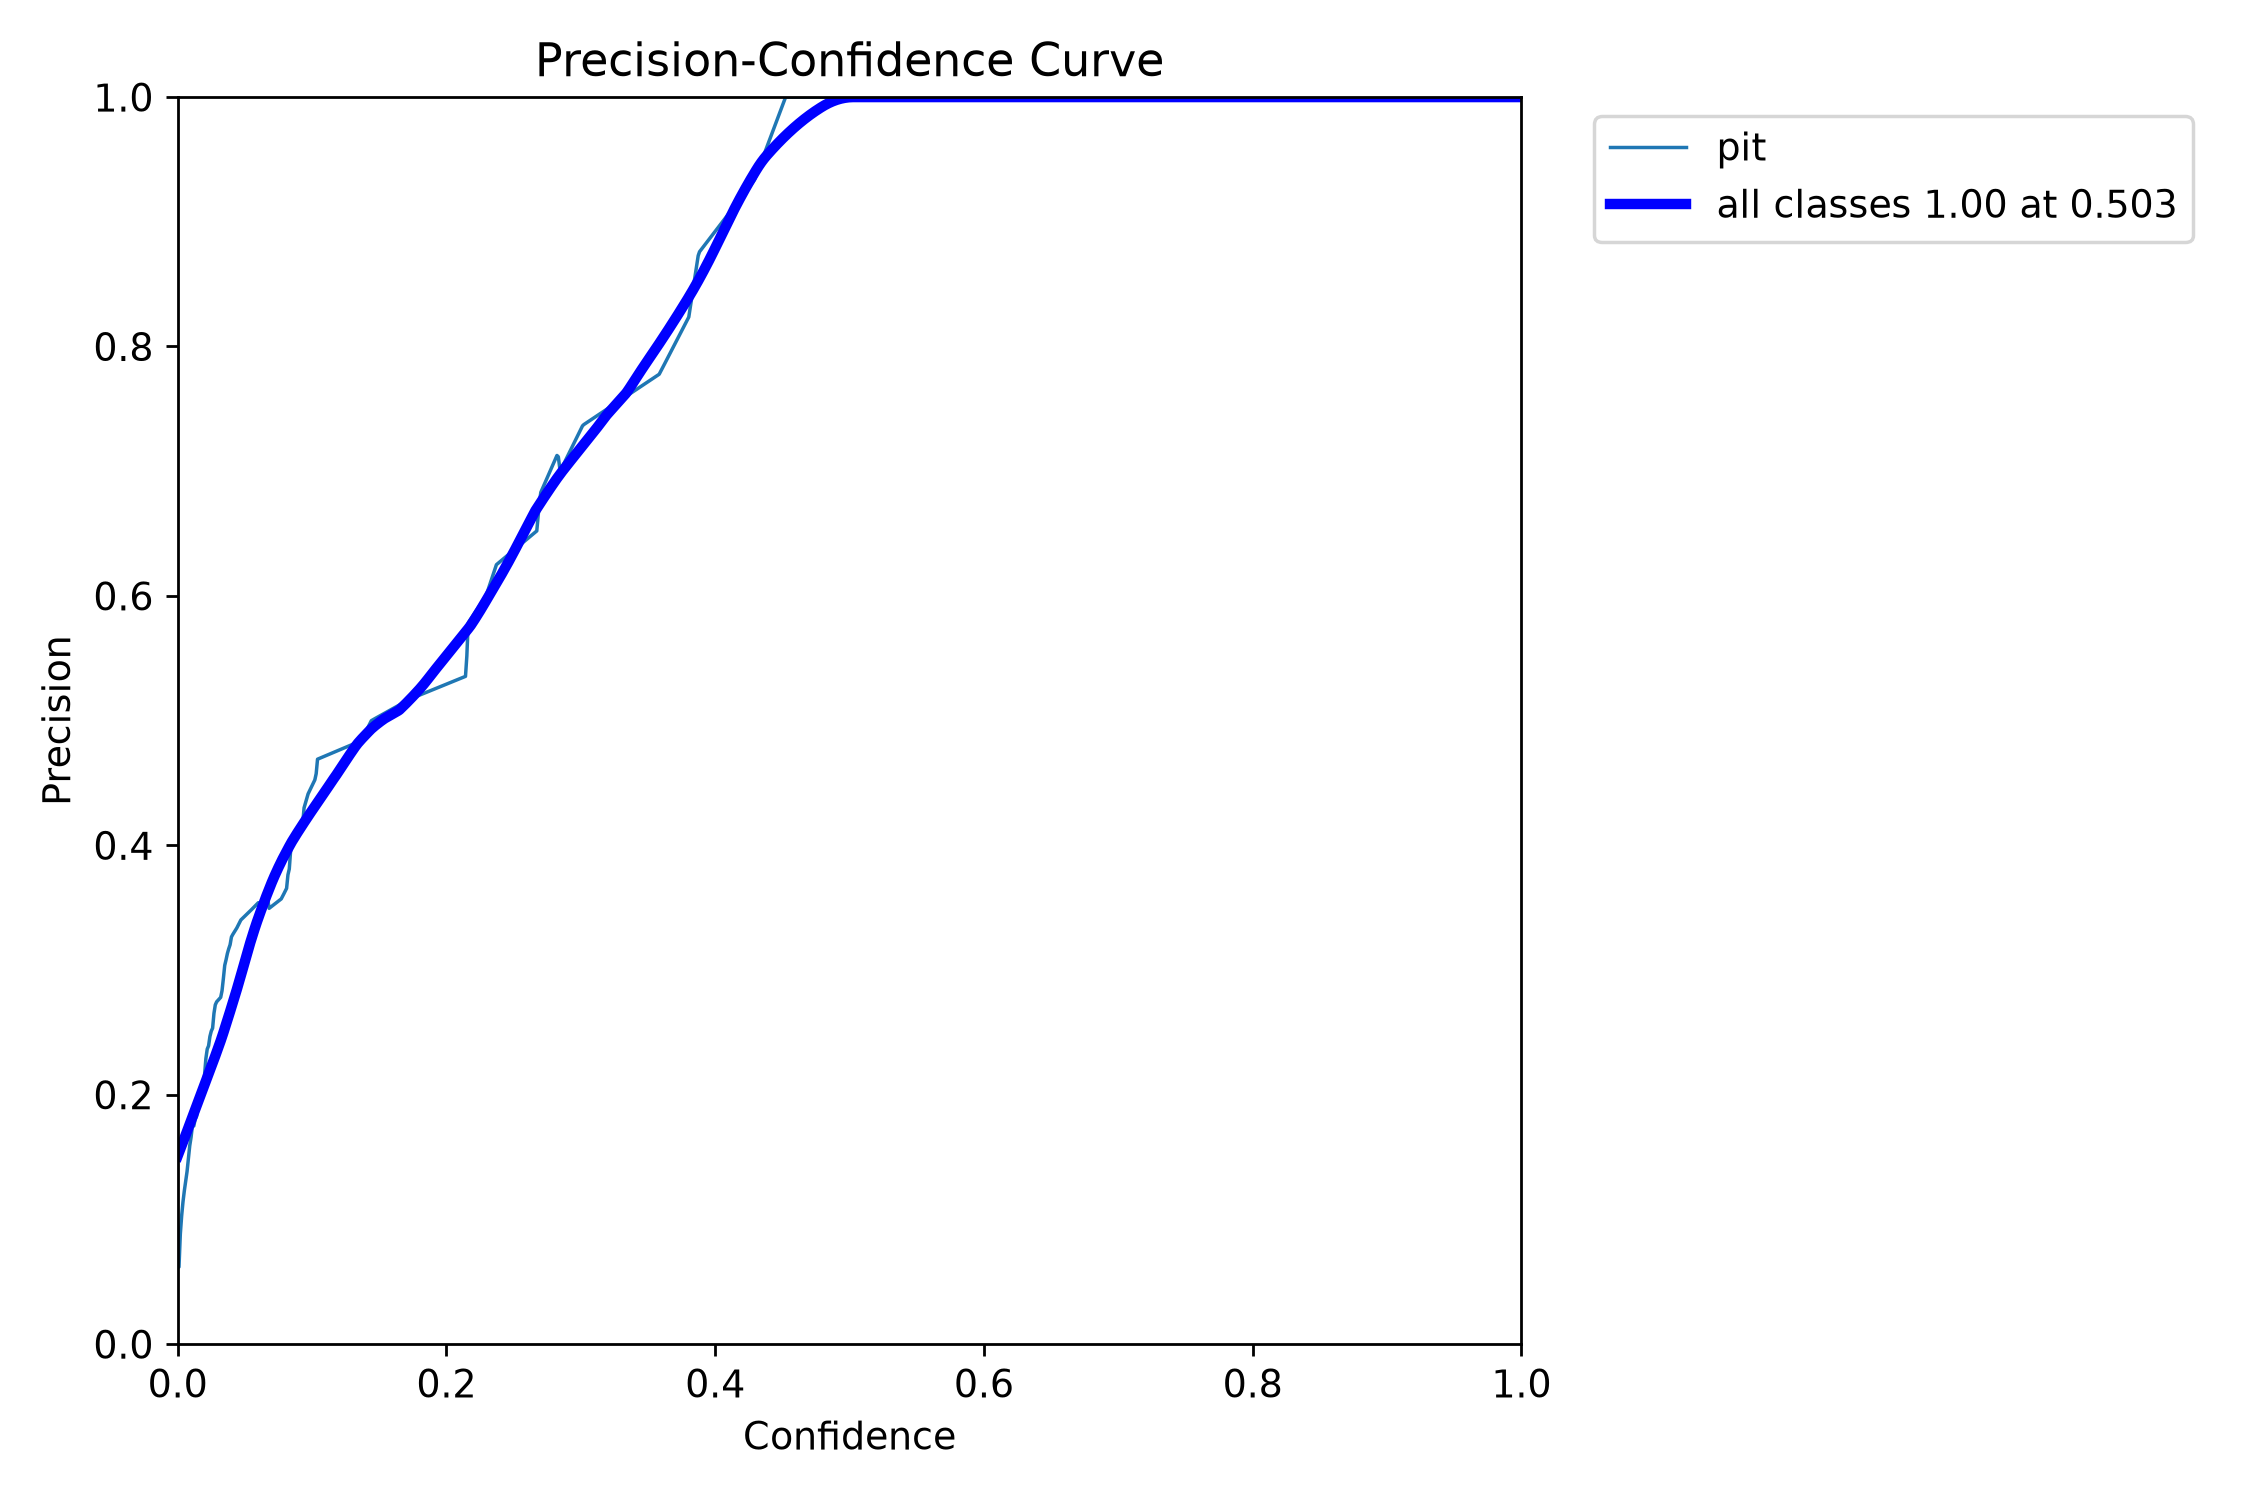
\includegraphics[width=\textwidth]{images/BoxP_curve.png}
    \caption{Precision vs. Confidence}
    \label{fig:sub-first}
  \end{subfigure}
  \hfill % Adds horizontal space between the two images
  \begin{subfigure}[b]{0.45\textwidth}
    \centering
    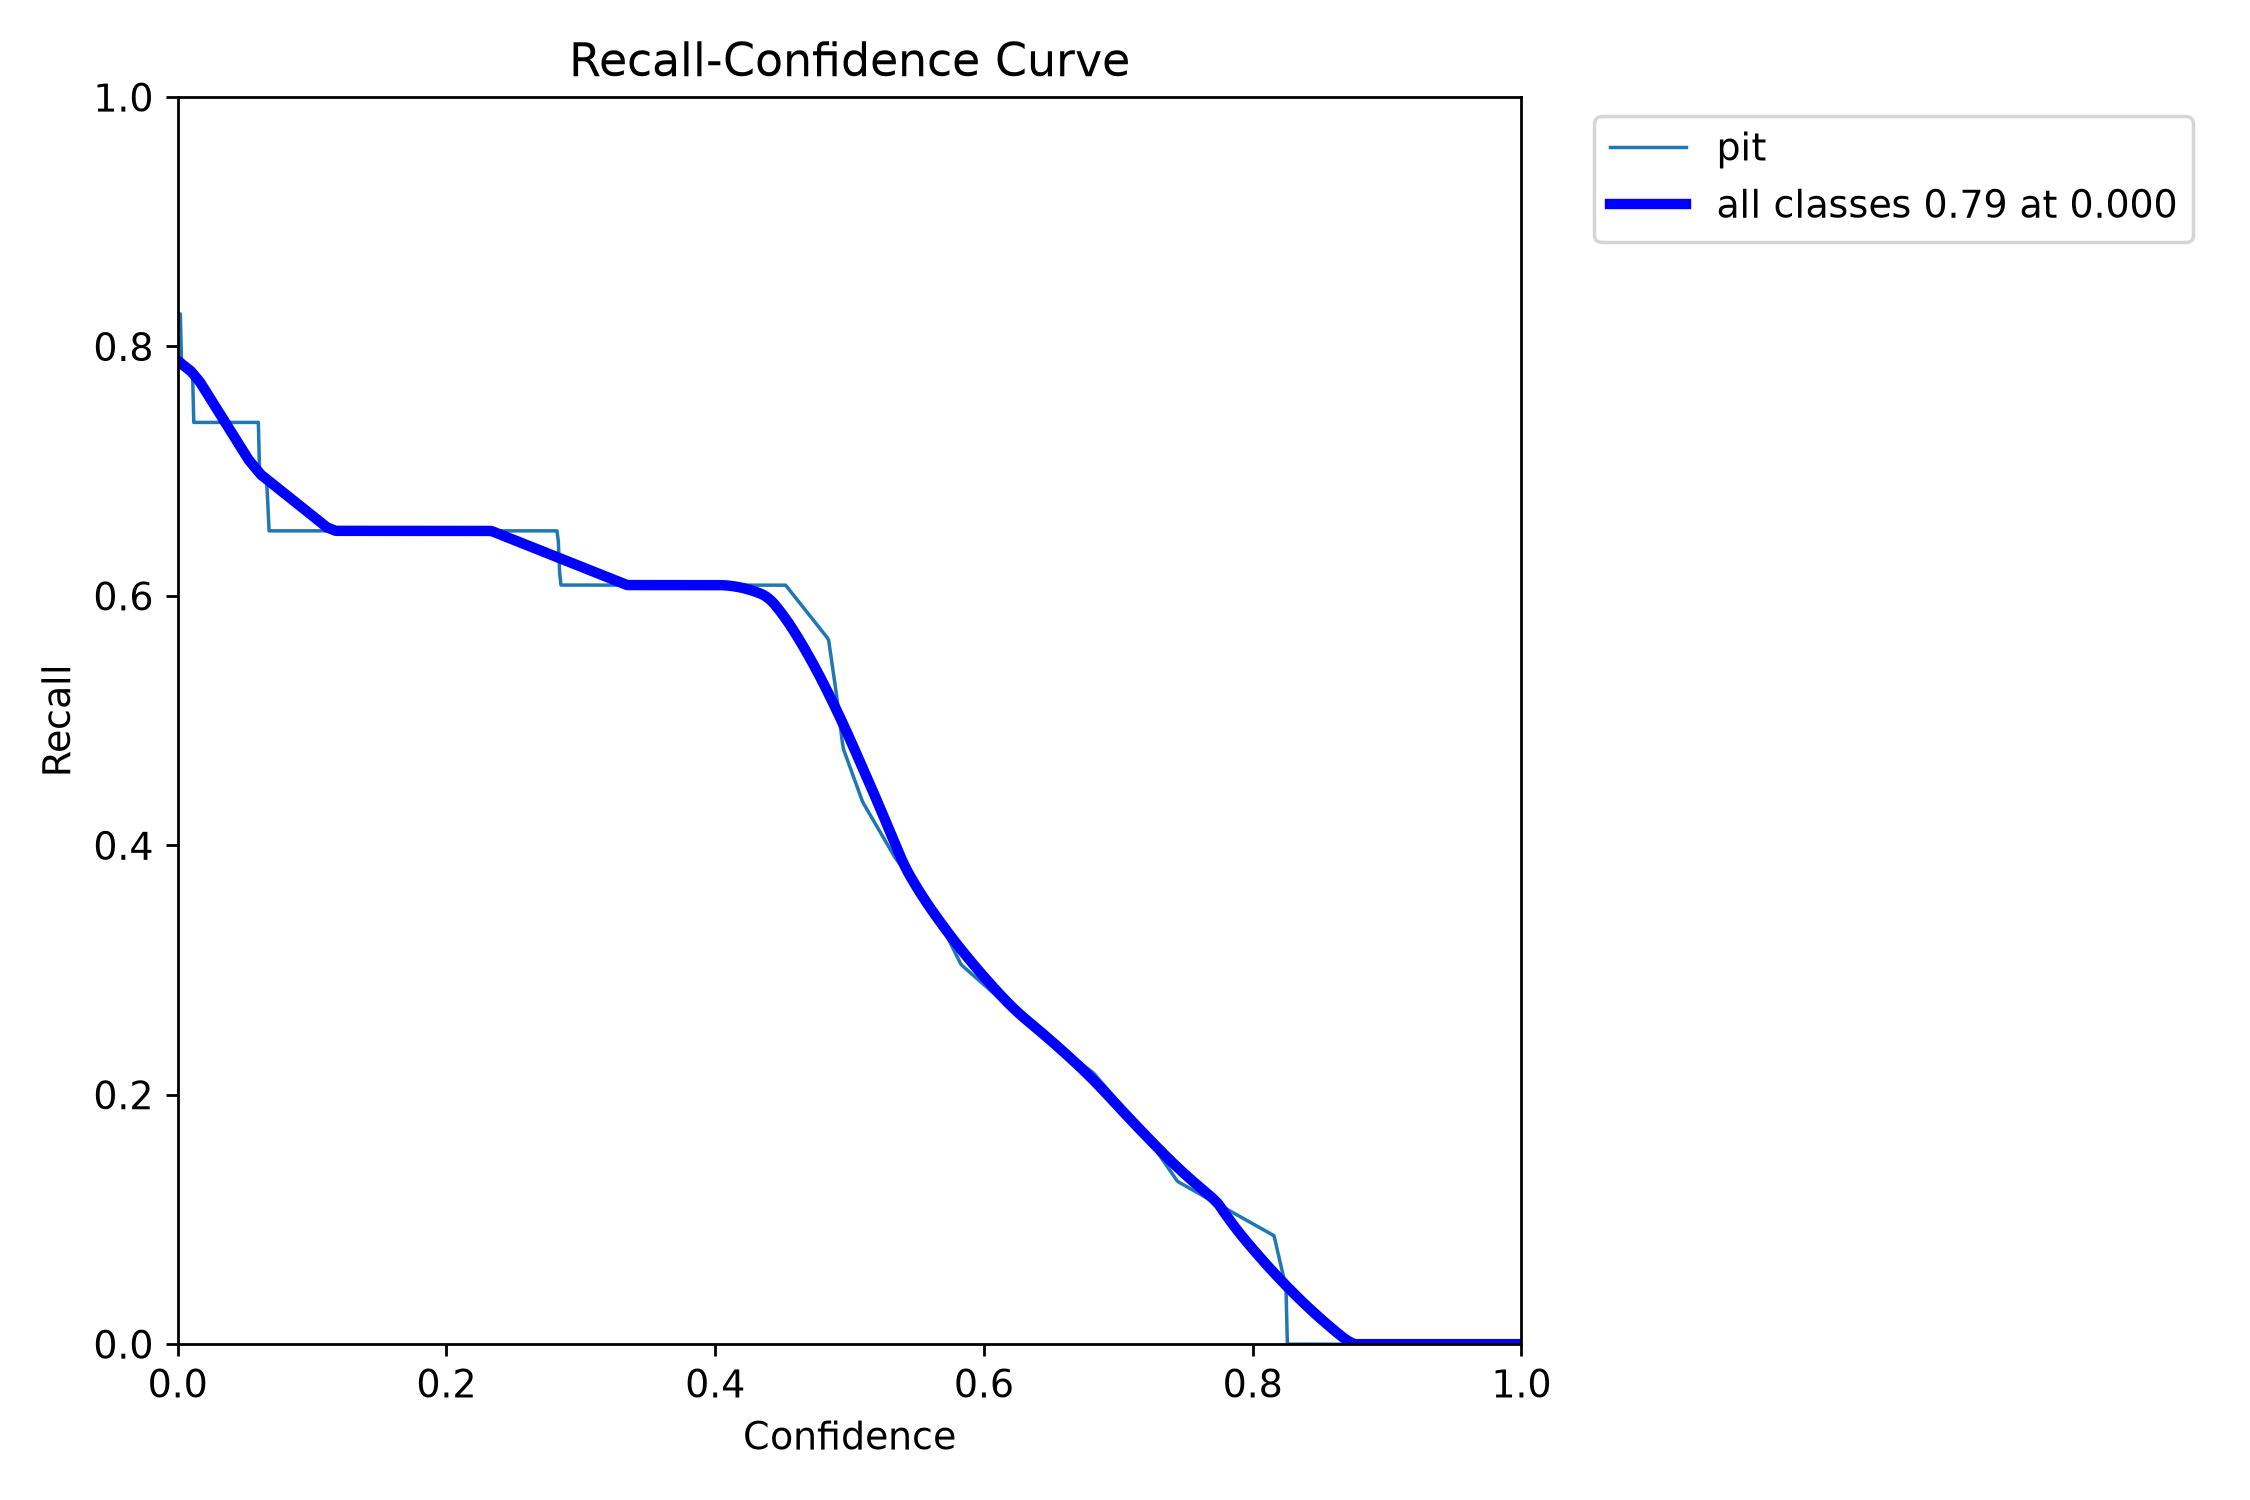
\includegraphics[width=\textwidth]{images/BoxR_curve.png}
    \caption{Recall vs. Confidence}
    \label{fig:sub-second}
  \end{subfigure}
  \label{fig:main-group}
\end{figure}

When inferences are run on new images, one of the arguments that can be passed into the model's prediction method is the confidence threshold. This is the confidence that is required for the model to label an image as a pit. Precision measures how many of the model's predictions were correct, while recall measures how many of the target classes, or pits, were identified by the model. Since precision and recall are inverses of each other and I want to balance the two, approximately 0.5 is a good confidence threshold to optimize each one for inferencing new images.

% \begin{table}[h]
% \centering
% \caption{Example table demonstrating the recommended table formatting.}
% \label{tab:example-table}
% \resizebox{\columnwidth}{!}{%
% \begin{tabular}{|c|c|c|}
% \hline
% \textbf{Category} & \textbf{Metric A} & \textbf{Metric B} \\
% \hline
% Group 1 & 0.85 & 12\% \\
% Group 2 & 0.78 & 10\% \\
% Group 3 & 0.65 & 8\% \\
% Group 4 & 0.50 & 5\% \\
% \hline
% \end{tabular}%
% }
% \end{table}

\section{Conclusion}
Before this project, there were about 250 pits previously identified. This meant that there were few images to create the dataset for training the model. However, 60\% is not a bad accuracy score, as the goal of this project was to identify lunar skylight candidates, not perfectly categorize geographical features. Even if the model misidentifies lunar pits, it's easier for a human to verify the predictions than to search for pits that the model glossed over.

\begin{figure}[htbp]
  \centering
  \begin{subfigure}[b]{0.45\textwidth}
    \centering
    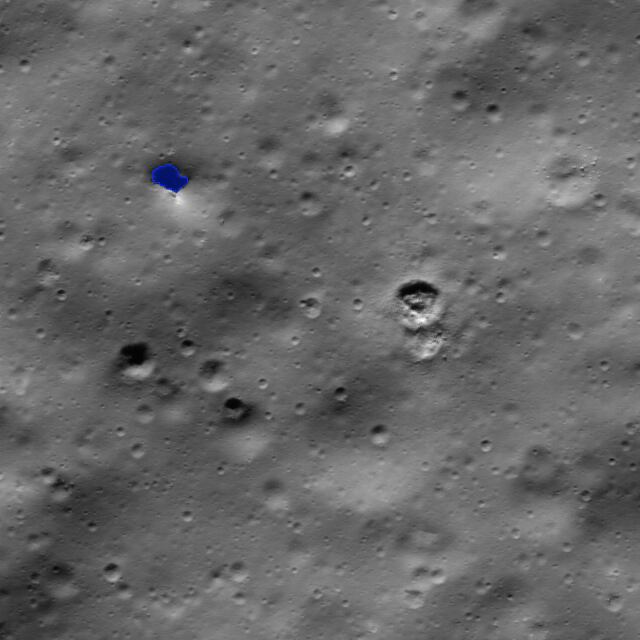
\includegraphics[width=\textwidth]{images/m154705713rc_cropped_masked.png}
    \caption{Column 1}
    \label{fig:sub-first}
  \end{subfigure}
  \hfill % Adds horizontal space between the two images
  \begin{subfigure}[b]{0.45\textwidth}
    \centering
    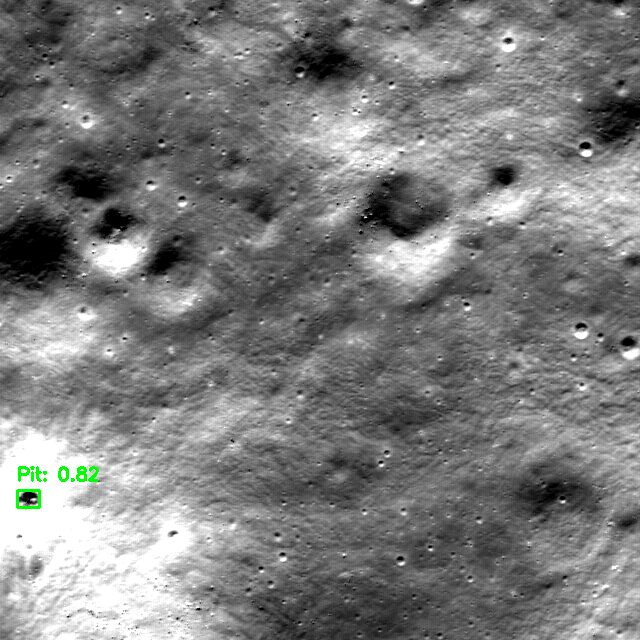
\includegraphics[width=\textwidth]{images/M187722274LC_600_9600.png}
    \caption{Column 2}
    \label{fig:sub-second}
  \end{subfigure}
  \label{fig:main-group}
\end{figure}

The two images above both show the same lunar pit, but in clearly different lighting conditions. The different lighting conditions are a result of the NAC taking pictures from different angles at different times of day, when the sun is also at a different angle. Although this isn't a possible type of image transformation for YOLO, the model was still able to figure out where the pit was in different locations. For a model trained on a dataset of approximately 150 images (including backgrounds), this is pretty good accuracy. Additionally, though the model made several false predictions of pits, it is important to remember that the images are approximately 5000x50000 pixels, or 2.5x25km. There are thousands of craters in each image, so only mistaking 8 of them for pits is a pretty good result.

In order to further hone the model's accuracy, I would run inferences on the column 2 and 3 images, then pass the bounding boxes back into the model. This would make the dataset more robust with more images to train on. Beyond that, since there aren't very many previously identified lunar pits, the model will inevitably not be able to train on many pit images. However, with the current model's accuracy, it's very possible to identify lunar pit candidates in images and then have humans review the images. It's better to falsely predict an image has a pit, as that would only waste a couple seconds per image, versus completely glossing over actual pits.

\section{Acknowledgements}
\fontsize{11}{13}\selectfont

% \textbf{Author Contribution:}
% [Describe each author's contribution, e.g., using CRediT taxonomy roles such as conceptualization
I would like to thank my mentor David Palmer for his guidance and advice during this process. I would also like to thank Doug Mandell for providing tech assistance and Mark Galassi for making this opportunity possible.

% Example for references section


\printbibliography  % Use BibLaTeX for printing bibliography

\end{document}
